%%%% Paramétrage du cours %%%%
\def\xxactivite{ Exercices d'application  }
\def\xxauteur{\textsl{Émilien Durif -- Xavier Pessoles}}

%\fichefalse
%\proftrue
%\tdfalse
%\courstrue

% Déclaration des titres
% -------------------------------------


\graphicspath{{../../style/png/}{images/}{../../exos//}}
\lstinputpath{{../../exos//}}

\def\discipline{Informatique}
\def\xxtete{Informatique}

\def\classe{\textsf{MPSI}}
\def\xxnumpartie{1}
\def\xxpartie{Architecture matérielle et initiation à l'algorithmique}
\def\xxdate{11 Décembre 2019}

\def\xxchapitre{08}
\def\xxnumchapitre{08}
\def\xxnomchapitre{Représentation des nombres}
\def\xxnumactivite{08}

\def\xxposongletx{2}
\def\xxposonglettext{1.45}
\def\xxposonglety{19}%16

\def\xxonglet{\textsf{Cycle 01}}
\def\xxauteur{\textsl{Émilien Durif -- Sylvaine Kleim \\ Xavier Pessoles }}


\def\xxpied{%
Cycle \xxnumpartie -- \xxpartie\\
Chapitre \xxnumchapitre -- \xxactivite -\xxnumactivite -- \xxnomchapitre%
}

\setcounter{secnumdepth}{5}
\chapterimage{Fond_ALG}
\def\xxfigures{}

\def\xxcompetences{%
\textsl{%
%\vspace{-.5cm}
\textbf{Savoirs et compétences :}\\
\vspace{-.1cm}
\begin{itemize}[label=\ding{112},font=\color{ocre}]
\item AA.C2 : Appréhender les limitations intrinsèques à la manipulation informatique des nombres
\item AA.C3 : Initier un sens critique au sujet de la qualité et de la précision des résultats de calculs numériques sur ordinateur
\item AA.S4 : Principe de la représentation des nombres entiers en mémoire
\item AA.S5 : Principe de la représentation des nombres réels en mémoire
\end{itemize}
}}


%Infos sur les supports
\def\xxtitreexo{Représentation des nombres}
\def\xxsourceexo{\hspace{.2cm} \footnotesize{
}}
%\def\xxtitreexo{Titre EXO}
%\def\xxsourceexo{\hspace{.2cm} \footnotesize{Source EXO}}


%---------------------------------------------------------------------------





\def\xxfigures{
%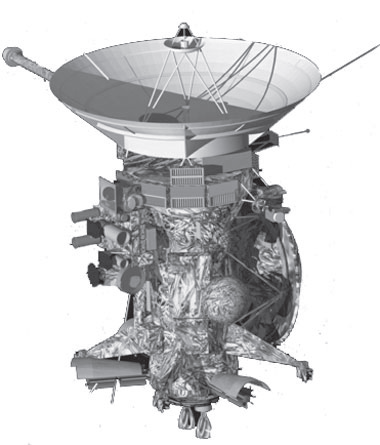
\includegraphics[width=.6\linewidth]{fig_00}
}%figues de la page de garde


\iflivret
\pagestyle{empty}


%%%%%%%% PAGE DE GARDE COURS
\ifcours
% ==== BANDEAU DES TITRES ==== 
\begin{tikzpicture}[remember picture,overlay]
\node at (current page.north west)
{\begin{tikzpicture}[remember picture,overlay]
\node[anchor=north west,inner sep=0pt] at (0,0) {\includegraphics[width=\paperwidth]{\thechapterimage}};
\draw[anchor=west] (-2cm,-8cm) node [line width=2pt,rounded corners=15pt,draw=ocre,fill=white,fill opacity=0.6,inner sep=40pt]{\strut\makebox[22cm]{}};
\draw[anchor=west] (1cm,-8cm) node {\huge\sffamily\bfseries\color{black} %
\begin{minipage}{1cm}
\rotatebox{90}{\LARGE\sffamily\textsc{\color{ocre}\textbf{\xxnumpartie}}}
\end{minipage} \hfill
\begin{minipage}[c]{14cm}
\begin{titrepartie}
\begin{flushright}
\renewcommand{\baselinestretch}{1.1} 
\Large\sffamily\textsc{\textbf{\xxpartie}}
\renewcommand{\baselinestretch}{1} 
\end{flushright}
\end{titrepartie}
\end{minipage} \hfill
\begin{minipage}[c]{3.5cm}
{\large\sffamily\textsc{\textbf{\color{ocre} \discipline}}}
\end{minipage} 
 };
\end{tikzpicture}};
\end{tikzpicture}
% ==== FIN BANDEAU DES TITRES ==== 


% ==== ONGLET 
\begin{tikzpicture}[overlay]
\node[shape=rectangle, 
      rounded corners = .25 cm,
	  draw= ocre,
	  line width=2pt, 
	  fill = ocre!10,
	  minimum width  = 2.5cm,
	  minimum height = 3cm,] at (18.3cm,0) {};
\node at (17.7cm,0) {\rotatebox{90}{\textbf{\Large\color{ocre}{\classe}}}};
%{};
\end{tikzpicture}
% ==== FIN ONGLET 


\vspace{3.5cm}

\begin{tikzpicture}[remember picture,overlay]
\draw[anchor=west] (-2cm,-6cm) node {\huge\sffamily\bfseries\color{black} %
\begin{minipage}{2cm}
\begin{center}
\LARGE\sffamily\textsc{\color{ocre}\textbf{\xxactivite}}
\end{center}
\end{minipage} \hfill
\begin{minipage}[c]{15cm}
\begin{titrechapitre}
\renewcommand{\baselinestretch}{1.1} 
%\Large\sffamily\textsc{\textbf{\xxnumchapitre}}
%
%\Large\sffamily\textsc{\textbf{\xxchapitre}}
\vspace{.5cm}

\renewcommand{\baselinestretch}{1} 
\normalsize\normalfont
\xxcompetences
\end{titrechapitre}
\end{minipage}  };
\end{tikzpicture}
\vfill

\begin{flushright}
\begin{minipage}[c]{.3\linewidth}
\begin{center}
\xxfigures
\end{center}
\end{minipage}\hfill
\begin{minipage}[c]{.6\linewidth}
\startcontents
%\printcontents{}{1}{}
\printcontents{}{1}{}
\end{minipage}
\end{flushright}

\begin{tikzpicture}[remember picture,overlay]
\draw[anchor=west] (4.5cm,-.7cm) node {
\begin{minipage}[c]{.2\linewidth}
\begin{flushright}

\includegraphics[width=2cm]{logoCC}
\end{flushright}
\end{minipage}
\begin{minipage}[c]{.2\linewidth}
\textsl{\xxauteur} \\
\textsl{\classe}
\end{minipage}
 };
\end{tikzpicture}

\newpage
\pagestyle{fancy}

%\newpage
%\pagestyle{fancy}

\else
\fi
%% FIN PAGE DE GARDE DES COURS

%%%%%%%% PAGE DE GARDE TD
\iftd
%\begin{tikzpicture}[remember picture,overlay]
%\node at (current page.north west)
%{\begin{tikzpicture}[remember picture,overlay]
%\draw[anchor=west] (-2cm,-3.25cm) node [line width=2pt,rounded corners=15pt,draw=ocre,fill=white,fill opacity=0.6,inner sep=40pt]{\strut\makebox[22cm]{}};
%\draw[anchor=west] (1cm,-3.25cm) node {\huge\sffamily\bfseries\color{black} %
%\begin{minipage}{1cm}
%\rotatebox{90}{\LARGE\sffamily\textsc{\color{ocre}\textbf{\xxnumpartie}}}
%\end{minipage} \hfill
%\begin{minipage}[c]{13.5cm}
%\begin{titrepartie}
%\begin{flushright}
%\renewcommand{\baselinestretch}{1.1} 
%\Large\sffamily\textsc{\textbf{\xxpartie}}
%\renewcommand{\baselinestretch}{1} 
%\end{flushright}
%\end{titrepartie}
%\end{minipage} \hfill
%\begin{minipage}[c]{3.5cm}
%{\large\sffamily\textsc{\textbf{\color{ocre} \discipline}}}
%\end{minipage} 
% };
%\end{tikzpicture}};
%\end{tikzpicture}

%%%%%%%%%% PAGE DE GARDE TD %%%%%%%%%%%%%%%
%\begin{tikzpicture}[overlay]
%\node[shape=rectangle, 
%      rounded corners = .25 cm,
%	  draw= ocre,
%	  line width=2pt, 
%	  fill = ocre!10,
%	  minimum width  = 2.5cm,
%	  minimum height = 2.5cm,] at (18.5cm,0) {};
%\node at (17.7cm,0) {\rotatebox{90}{\textbf{\Large\color{ocre}{\classe}}}};
%%{};
%\end{tikzpicture}

% PARTIE ET CHAPITRE
%\begin{tikzpicture}[remember picture,overlay]
%\draw[anchor=west] (-1cm,-2.1cm) node {\large\sffamily\bfseries\color{black} %
%\begin{minipage}[c]{15cm}
%\begin{flushleft}
%\xxnumchapitre \\
%\xxchapitre
%\end{flushleft}
%\end{minipage}  };
%\end{tikzpicture}

% BANDEAU EXO
\iflivret % SI LIVRET
\begin{tikzpicture}[remember picture,overlay]
\draw[anchor=west] (-2cm,-3.3cm) node {\huge\sffamily\bfseries\color{black} %
\begin{minipage}{5cm}
\begin{center}
\LARGE\sffamily\color{ocre}\textbf{\textsc{\xxactivite}}

\begin{center}
\xxfigures
\end{center}

\end{center}
\end{minipage} \hfill
\begin{minipage}[c]{12cm}
\begin{titrechapitre}
\renewcommand{\baselinestretch}{1.1} 
\large\sffamily\textbf{\textsc{\xxtitreexo}}

\small\sffamily{\textbf{\textit{\color{black!70}\xxsourceexo}}}
\vspace{.5cm}

\renewcommand{\baselinestretch}{1} 
\normalsize\normalfont
\xxcompetences
\end{titrechapitre}
\end{minipage}};
\end{tikzpicture}
\else % ELSE NOT LIVRET
\begin{tikzpicture}[remember picture,overlay]
\draw[anchor=west] (-2cm,-4.5cm) node {\huge\sffamily\bfseries\color{black} %
\begin{minipage}{5cm}
\begin{center}
\LARGE\sffamily\color{ocre}\textbf{\textsc{\xxactivite}}

\begin{center}
\xxfigures
\end{center}

\end{center}
\end{minipage} \hfill
\begin{minipage}[c]{12cm}
\begin{titrechapitre}
\renewcommand{\baselinestretch}{1.1} 
\large\sffamily\textbf{\textsc{\xxtitreexo}}

\small\sffamily{\textbf{\textit{\color{black!70}\xxsourceexo}}}
\vspace{.5cm}

\renewcommand{\baselinestretch}{1} 
\normalsize\normalfont
\xxcompetences
\end{titrechapitre}
\end{minipage}};
\end{tikzpicture}

\fi

\else   % FIN IF TD
\fi


%%%%%%%% PAGE DE GARDE FICHE
\iffiche
\begin{tikzpicture}[remember picture,overlay]
\node at (current page.north west)
{\begin{tikzpicture}[remember picture,overlay]
\draw[anchor=west] (-2cm,-2.25cm) node [line width=2pt,rounded corners=15pt,draw=ocre,fill=white,fill opacity=0.6,inner sep=40pt]{\strut\makebox[22cm]{}};
\draw[anchor=west] (1cm,-2.25cm) node {\huge\sffamily\bfseries\color{black} %
\begin{minipage}{1cm}
\rotatebox{90}{\LARGE\sffamily\textsc{\color{ocre}\textbf{\xxnumpartie}}}
\end{minipage} \hfill
\begin{minipage}[c]{14cm}
\begin{titrepartie}
\begin{flushright}
\renewcommand{\baselinestretch}{1.1} 
\large\sffamily\textsc{\textbf{\xxpartie} \\} 

\vspace{.2cm}

\normalsize\sffamily\textsc{\textbf{\xxnumchapitre -- \xxchapitre}}
\renewcommand{\baselinestretch}{1} 
\end{flushright}
\end{titrepartie}
\end{minipage} \hfill
\begin{minipage}[c]{3.5cm}
{\large\sffamily\textsc{\textbf{\color{ocre} \discipline}}}
\end{minipage} 
 };
\end{tikzpicture}};
\end{tikzpicture}

\iflivret
\begin{tikzpicture}[overlay]
\node[shape=rectangle, 
      rounded corners = .25 cm,
	  draw= ocre,
	  line width=2pt, 
	  fill = ocre!10,
	  minimum width  = 2.5cm,
	  minimum height = 2.5cm,] at (18.5cm,1.1cm) {};
\node at (17.9cm,1.1cm) {\rotatebox{90}{\textsf{\textbf{\large\color{ocre}{\classe}}}}};
%{};
\end{tikzpicture}
\else
\begin{tikzpicture}[overlay]
\node[shape=rectangle, 
      rounded corners = .25 cm,
	  draw= ocre,
	  line width=2pt, 
	  fill = ocre!10,
	  minimum width  = 2.5cm,
%	  minimum height = 2.5cm,] at (18.5cm,1.1cm) {};
	  minimum height = 2.5cm,] at (18.6cm,0cm) {};
\node at (18cm,0cm) {\rotatebox{90}{\textsf{\textbf{\large\color{ocre}{\classe}}}}};
%{};
\end{tikzpicture}

\fi

\else
\fi



\else
\pagestyle{empty}


%%%%%%%% PAGE DE GARDE COURS
\ifcours
% ==== BANDEAU DES TITRES ==== 
\begin{tikzpicture}[remember picture,overlay]
\node at (current page.north west)
{\begin{tikzpicture}[remember picture,overlay]
\node[anchor=north west,inner sep=0pt] at (0,0) {\includegraphics[width=\paperwidth]{\thechapterimage}};
\draw[anchor=west] (-2cm,-8cm) node [line width=2pt,rounded corners=15pt,draw=ocre,fill=white,fill opacity=0.6,inner sep=40pt]{\strut\makebox[22cm]{}};
\draw[anchor=west] (1cm,-8cm) node {\huge\sffamily\bfseries\color{black} %
\begin{minipage}{1cm}
\rotatebox{90}{\LARGE\sffamily\textsc{\color{ocre}\textbf{\xxnumpartie}}}
\end{minipage} \hfill
\begin{minipage}[c]{14cm}
\begin{titrepartie}
\begin{flushright}
\renewcommand{\baselinestretch}{1.1} 
\Large\sffamily\textsc{\textbf{\xxpartie}}
\renewcommand{\baselinestretch}{1} 
\end{flushright}
\end{titrepartie}
\end{minipage} \hfill
\begin{minipage}[c]{3.5cm}
{\large\sffamily\textsc{\textbf{\color{ocre} \discipline}}}
\end{minipage} 
 };
\end{tikzpicture}};
\end{tikzpicture}
% ==== FIN BANDEAU DES TITRES ==== 


% ==== ONGLET 
\begin{tikzpicture}[overlay]
\node[shape=rectangle, 
      rounded corners = .25 cm,
	  draw= ocre,
	  line width=2pt, 
	  fill = ocre!10,
	  minimum width  = 2.5cm,
	  minimum height = 3cm,] at (18.3cm,0) {};
\node at (17.7cm,0) {\rotatebox{90}{\textbf{\Large\color{ocre}{\classe}}}};
%{};
\end{tikzpicture}
% ==== FIN ONGLET 


\vspace{3.5cm}

\begin{tikzpicture}[remember picture,overlay]
\draw[anchor=west] (-2cm,-6cm) node {\huge\sffamily\bfseries\color{black} %
\begin{minipage}{2cm}
\begin{center}
\LARGE\sffamily\textsc{\color{ocre}\textbf{\xxactivite}}
\end{center}
\end{minipage} \hfill
\begin{minipage}[c]{15cm}
\begin{titrechapitre}
\renewcommand{\baselinestretch}{1.1} 
%\Large\sffamily\textsc{\textbf{\xxnumchapitre}}
%
%\Large\sffamily\textsc{\textbf{\xxchapitre}}
\vspace{.5cm}

\renewcommand{\baselinestretch}{1} 
\normalsize\normalfont
\xxcompetences
\end{titrechapitre}
\end{minipage}  };
\end{tikzpicture}
\vfill

\begin{flushright}
\begin{minipage}[c]{.3\linewidth}
\begin{center}
\xxfigures
\end{center}
\end{minipage}\hfill
\begin{minipage}[c]{.6\linewidth}
\startcontents
%\printcontents{}{1}{}
\printcontents{}{1}{}
\end{minipage}
\end{flushright}

\begin{tikzpicture}[remember picture,overlay]
\draw[anchor=west] (4.5cm,-.7cm) node {
\begin{minipage}[c]{.2\linewidth}
\begin{flushright}

\includegraphics[width=2cm]{logoCC}
\end{flushright}
\end{minipage}
\begin{minipage}[c]{.2\linewidth}
\textsl{\xxauteur} \\
\textsl{\classe}
\end{minipage}
 };
\end{tikzpicture}

\newpage
\pagestyle{fancy}

%\newpage
%\pagestyle{fancy}

\else
\fi
%% FIN PAGE DE GARDE DES COURS

%%%%%%%% PAGE DE GARDE TD
\iftd
%\begin{tikzpicture}[remember picture,overlay]
%\node at (current page.north west)
%{\begin{tikzpicture}[remember picture,overlay]
%\draw[anchor=west] (-2cm,-3.25cm) node [line width=2pt,rounded corners=15pt,draw=ocre,fill=white,fill opacity=0.6,inner sep=40pt]{\strut\makebox[22cm]{}};
%\draw[anchor=west] (1cm,-3.25cm) node {\huge\sffamily\bfseries\color{black} %
%\begin{minipage}{1cm}
%\rotatebox{90}{\LARGE\sffamily\textsc{\color{ocre}\textbf{\xxnumpartie}}}
%\end{minipage} \hfill
%\begin{minipage}[c]{13.5cm}
%\begin{titrepartie}
%\begin{flushright}
%\renewcommand{\baselinestretch}{1.1} 
%\Large\sffamily\textsc{\textbf{\xxpartie}}
%\renewcommand{\baselinestretch}{1} 
%\end{flushright}
%\end{titrepartie}
%\end{minipage} \hfill
%\begin{minipage}[c]{3.5cm}
%{\large\sffamily\textsc{\textbf{\color{ocre} \discipline}}}
%\end{minipage} 
% };
%\end{tikzpicture}};
%\end{tikzpicture}

%%%%%%%%%% PAGE DE GARDE TD %%%%%%%%%%%%%%%
%\begin{tikzpicture}[overlay]
%\node[shape=rectangle, 
%      rounded corners = .25 cm,
%	  draw= ocre,
%	  line width=2pt, 
%	  fill = ocre!10,
%	  minimum width  = 2.5cm,
%	  minimum height = 2.5cm,] at (18.5cm,0) {};
%\node at (17.7cm,0) {\rotatebox{90}{\textbf{\Large\color{ocre}{\classe}}}};
%%{};
%\end{tikzpicture}

% PARTIE ET CHAPITRE
%\begin{tikzpicture}[remember picture,overlay]
%\draw[anchor=west] (-1cm,-2.1cm) node {\large\sffamily\bfseries\color{black} %
%\begin{minipage}[c]{15cm}
%\begin{flushleft}
%\xxnumchapitre \\
%\xxchapitre
%\end{flushleft}
%\end{minipage}  };
%\end{tikzpicture}

% BANDEAU EXO
\iflivret % SI LIVRET
\begin{tikzpicture}[remember picture,overlay]
\draw[anchor=west] (-2cm,-3.3cm) node {\huge\sffamily\bfseries\color{black} %
\begin{minipage}{5cm}
\begin{center}
\LARGE\sffamily\color{ocre}\textbf{\textsc{\xxactivite}}

\begin{center}
\xxfigures
\end{center}

\end{center}
\end{minipage} \hfill
\begin{minipage}[c]{12cm}
\begin{titrechapitre}
\renewcommand{\baselinestretch}{1.1} 
\large\sffamily\textbf{\textsc{\xxtitreexo}}

\small\sffamily{\textbf{\textit{\color{black!70}\xxsourceexo}}}
\vspace{.5cm}

\renewcommand{\baselinestretch}{1} 
\normalsize\normalfont
\xxcompetences
\end{titrechapitre}
\end{minipage}};
\end{tikzpicture}
\else % ELSE NOT LIVRET
\begin{tikzpicture}[remember picture,overlay]
\draw[anchor=west] (-2cm,-4.5cm) node {\huge\sffamily\bfseries\color{black} %
\begin{minipage}{5cm}
\begin{center}
\LARGE\sffamily\color{ocre}\textbf{\textsc{\xxactivite}}

\begin{center}
\xxfigures
\end{center}

\end{center}
\end{minipage} \hfill
\begin{minipage}[c]{12cm}
\begin{titrechapitre}
\renewcommand{\baselinestretch}{1.1} 
\large\sffamily\textbf{\textsc{\xxtitreexo}}

\small\sffamily{\textbf{\textit{\color{black!70}\xxsourceexo}}}
\vspace{.5cm}

\renewcommand{\baselinestretch}{1} 
\normalsize\normalfont
\xxcompetences
\end{titrechapitre}
\end{minipage}};
\end{tikzpicture}

\fi

\else   % FIN IF TD
\fi


%%%%%%%% PAGE DE GARDE FICHE
\iffiche
\begin{tikzpicture}[remember picture,overlay]
\node at (current page.north west)
{\begin{tikzpicture}[remember picture,overlay]
\draw[anchor=west] (-2cm,-2.25cm) node [line width=2pt,rounded corners=15pt,draw=ocre,fill=white,fill opacity=0.6,inner sep=40pt]{\strut\makebox[22cm]{}};
\draw[anchor=west] (1cm,-2.25cm) node {\huge\sffamily\bfseries\color{black} %
\begin{minipage}{1cm}
\rotatebox{90}{\LARGE\sffamily\textsc{\color{ocre}\textbf{\xxnumpartie}}}
\end{minipage} \hfill
\begin{minipage}[c]{14cm}
\begin{titrepartie}
\begin{flushright}
\renewcommand{\baselinestretch}{1.1} 
\large\sffamily\textsc{\textbf{\xxpartie} \\} 

\vspace{.2cm}

\normalsize\sffamily\textsc{\textbf{\xxnumchapitre -- \xxchapitre}}
\renewcommand{\baselinestretch}{1} 
\end{flushright}
\end{titrepartie}
\end{minipage} \hfill
\begin{minipage}[c]{3.5cm}
{\large\sffamily\textsc{\textbf{\color{ocre} \discipline}}}
\end{minipage} 
 };
\end{tikzpicture}};
\end{tikzpicture}

\iflivret
\begin{tikzpicture}[overlay]
\node[shape=rectangle, 
      rounded corners = .25 cm,
	  draw= ocre,
	  line width=2pt, 
	  fill = ocre!10,
	  minimum width  = 2.5cm,
	  minimum height = 2.5cm,] at (18.5cm,1.1cm) {};
\node at (17.9cm,1.1cm) {\rotatebox{90}{\textsf{\textbf{\large\color{ocre}{\classe}}}}};
%{};
\end{tikzpicture}
\else
\begin{tikzpicture}[overlay]
\node[shape=rectangle, 
      rounded corners = .25 cm,
	  draw= ocre,
	  line width=2pt, 
	  fill = ocre!10,
	  minimum width  = 2.5cm,
%	  minimum height = 2.5cm,] at (18.5cm,1.1cm) {};
	  minimum height = 2.5cm,] at (18.6cm,0cm) {};
\node at (18cm,0cm) {\rotatebox{90}{\textsf{\textbf{\large\color{ocre}{\classe}}}}};
%{};
\end{tikzpicture}

\fi

\else
\fi



\fi
\setlength{\columnseprule}{.1pt}

\pagestyle{fancy}
\thispagestyle{plain}

\ifprof
\vspace{4.5cm}
\else
\vspace{4.5cm}
\fi

\def\columnseprulecolor{\color{ocre}}
\setlength{\columnseprule}{0.4pt} 

%%%%%%%%%%%%%%%%%%%%%%%

\setcounter{exo}{0}
\vspace{2cm}
\begin{multicols}{2}

\subsection*{Comparaison des méthodes de résolution}


Soit l'équation \emph{E} : \quad $x\ln(x)=1$ .

On admet (si un doute vérifiez-le rapidement) que \emph{E} admet une unique solution $\alpha$ sur $\mathbb R$ et que
$\alpha\in[1;\text{e}]$. On prendra e$\approx2.8$. On peut aussi noter qu'en python \texttt{e} est un attribut de la bibliothèque \texttt{math}. On y a donc accès par \texttt{math.e}.



\paragraph*{Méthode de dichotomie}

%
%\begin{minipage}[c]{.47\linewidth}
%
%\subparagraph{} \textit{Complétez la fonction ci-contre renvoyant une valeur approchée à \texttt{epsilon} près de cette solution par dichotomie.}
\subparagraph{} \textit{Vérifier qu'à 10$^{-6}$ près : $\alpha\approx 1.763223$ .}
\subparagraph{} \textit{Modifier cette fonction afin qu'elle affiche le nombre de répétition de la boucle.}
%\begin{py}

%\begin{minipage}{\linewidth}
%\ttfamily
%
%def dichotomie(f,epsilon):
%
%\rule{4ex}{0pt} a=\ldots
%
%\rule{4ex}{0pt} b=\ldots
%
%\rule{4ex}{0pt} while abs(\ldots
%
%\rule{8ex}{0pt} c=(a+b)/2
%
%\rule{8ex}{0pt} if f(a)*f(c) < 0 :
%
%\rule{12ex}{0pt} \ldots =c
%
%\rule{8ex}{0pt} else :
%
%\rule{12ex}{0pt} \ldots =c
%
%\rule{4ex}{0pt} return \ldots
%\end{minipage}
%
%\medskip\normalfont
%
%\end{py}
%%\end{minipage} 




\paragraph*{Méthode des cordes (Lagrange)}


\subparagraph{} \textit{À partir de la fonction précédente, créer une nouvelle fonction nommée \texttt{lagrange} renvoyant une valeur approchée à \texttt{epsilon} près de cette solution par la méthode des cordes (dite de Lagrange).}

\subparagraph{} \textit{Affichez le nombre de répétition de la boucle. Comparer avec la méthode précédente.}




\paragraph*{Méthode de Newton}
%\vspace{.25cm}
%
%\begin{minipage}[c]{.47\linewidth}

On souhaite comparer avec la méthode Newton, mais le test d'arrêt ne permet pas d'obtenir une valeur approchée avec un précision donnée. Nous allons donc nous servir des résultats précédents.

\texttt{f} et \texttt{fp} étant des fonctions saisies en python, et correspondant à $f$ et $f'$ alors l'algorithme de Newton est donné ci-contre.


\subparagraph{} \textit{Implémenter la méthode de Newton dans une fonction nommée \texttt{newton}. }

\subparagraph{} \textit{Comparer les méthodes. }

%\end{minipage} \hfill
%\begin{minipage}[c]{.47\linewidth}
%\begin{py}
%\ttfamily
%x=2.8
%
%compteur=0 
%
%while abs(x-1.763223)>10**(-6):
%
%\rule{4ex}{0pt} x=\ldots
%
%\rule{4ex}{0pt} compteur=\ldots
%
%print(compteur)
%
%\end{py}
%\end{minipage} 


\setcounter{subparagraph}{0}



\subsection*{Suite définie implicitement}

Soit $f_n$ une suite de fonction définie sur $\mathbb R$ pour tout $n\in\mathbb N^*$ tel que :

\hfil $f_n(x)=x^n+x^{n-1}+x-1$

\subparagraph{} \textit{ Montrer que, pour tout $n\in\mathbb N^*$, l'équation $f_n(x)=0$ possède une unique solution sur $[0;1]$.}

\medskip

Notons $u_n$ cette solution.

\subparagraph{} \textit{\'Ecrire un programme Python qui :
\begin{itemize}
\item définit une fonction \texttt{f(x,n)} renvoyant la valeur $f_n(x)$;
\item définit une fonction \texttt{dichotomie(f,n)} renvoyant un valeur à $10^{-3}$ près de $u_n$;
\item calcule et affiche les 100 premières valeurs approchées de $(u_n)$.
\end{itemize}}

\subparagraph{} \textit{Conjecturer du comportement de cette suite.}


\newpage

\setcounter{exo}{0}

\subsection*{Les délices empoisonnés de la méthode de Newton}

\paragraph*{Partie A}

%\begin{minipage}[c]{.57\linewidth}
L'interprétation graphique de la méthode de Newton est donnée ci-contre.

Supposons que les fonctions $f$ et $f'$ soient définies en entête du programme.

\subparagraph{}\textit{Calculer les 20 premières valeurs de la suite générée par la méthode de Newton.}
%
%\begin{pseudo}
%
%\ttfamily
%
%\rule{0pt}{1.5em}
%x = x$_0$\\
%pour k allant de 1 à 20 faire :\\
%\rule{1cm}{0pt} x =
%\end{pseudo}
%
%
%\end{minipage} \hfill
%\begin{minipage}[c]{.4\linewidth}
\begin{center}
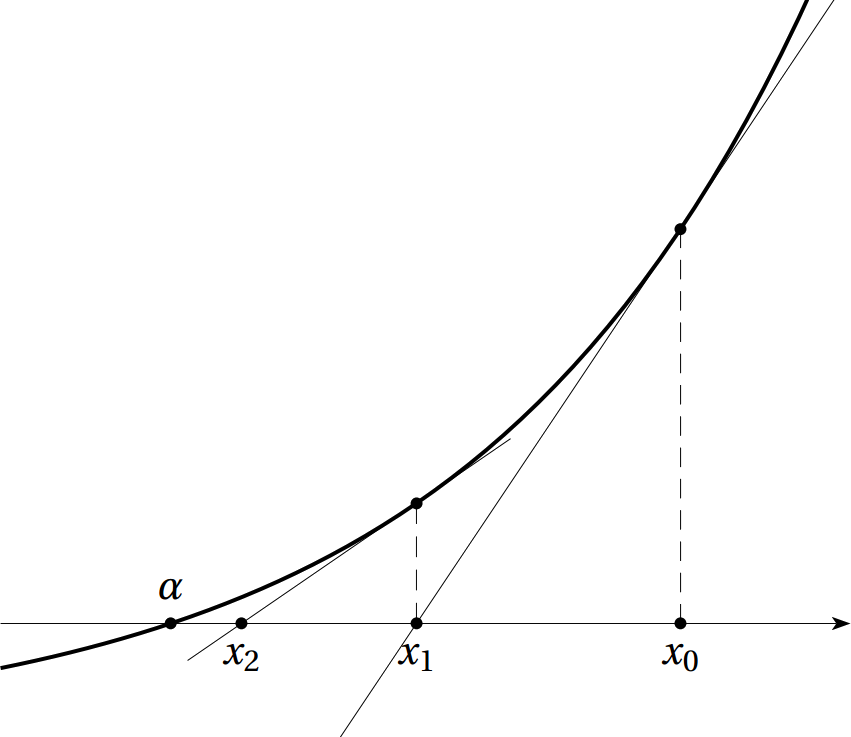
\includegraphics[width=\linewidth]{images/fig1}
\end{center}
%\end{minipage}

%\psset{xunit=1.5cm,yunit=1.0cm,algebraic=true,dimen=middle,dotstyle=o,dotsize=3pt 0,linewidth=0.2pt,arrowsize=3pt 2,arrowinset=0.25}
%\begin{pspicture*}(-1.,-1.)(4.,5.5)
%%\psaxes[labelFontSize=\scriptstyle,xAxis=true,yAxis=true,Dx=1.,Dy=1.,ticksize=-2pt 0,subticks=2]{->}(0,0)(-1.,-1.)(4.,5.5)
%\psline{->}(-1.,0)(4.,0)
%\psplot[linewidth=1pt]{-1.}{4.}{-1+2.71828^(0.5*x)}
%\psplot{-1.}{4.}{-3.2408445351690327+2.2408445351690323*x}
%\psplot{.1}{2}{(-0.4294061482447453+1.0304369953425587*x)}
%\psset{linestyle=dashed}
%\psline(1.4462603202968598,0.)(1.4462603202968598,1.0608739906851175)
%\psline(3.,0.)(3.,3.4816890703380645)
%%\begin{scriptsize}
%\psdots[dotstyle=*](0,0)(3.,0.)(3.,3.4816890703380645)(1.4462603202968598,0.)(1.4462603202968598,1.0608739906851175)(0.4167223713682693,0.)
%\rput(0,.3){$\alpha$}
%\rput(3,-.3){$x_0$}
%\rput(1.4462603202968598,-.3){$x_1$}
%\rput(0.4167223713682693,-.3){$x_2$}
%%\end{scriptsize}
%\end{pspicture*}

\paragraph*{Partie B}

Soit la fonction $f$ définie sur $\mathbb R$ par :\quad
$f(x) = x^3 - x^2 - 20x - 12$.



Considérons la suite définie par la méthode de Newton en partant de $x_0=2$

\subparagraph{}\textit{Écrire un programme en Python qui :
\begin{itemize}
\item définit la fonction $f$ ainsi que sa fonction dérivée que vous noterez $fp$,
\item calcule et affiche les valeurs successives de l'algorithme de Newton.
\end{itemize}}


\begin{center}
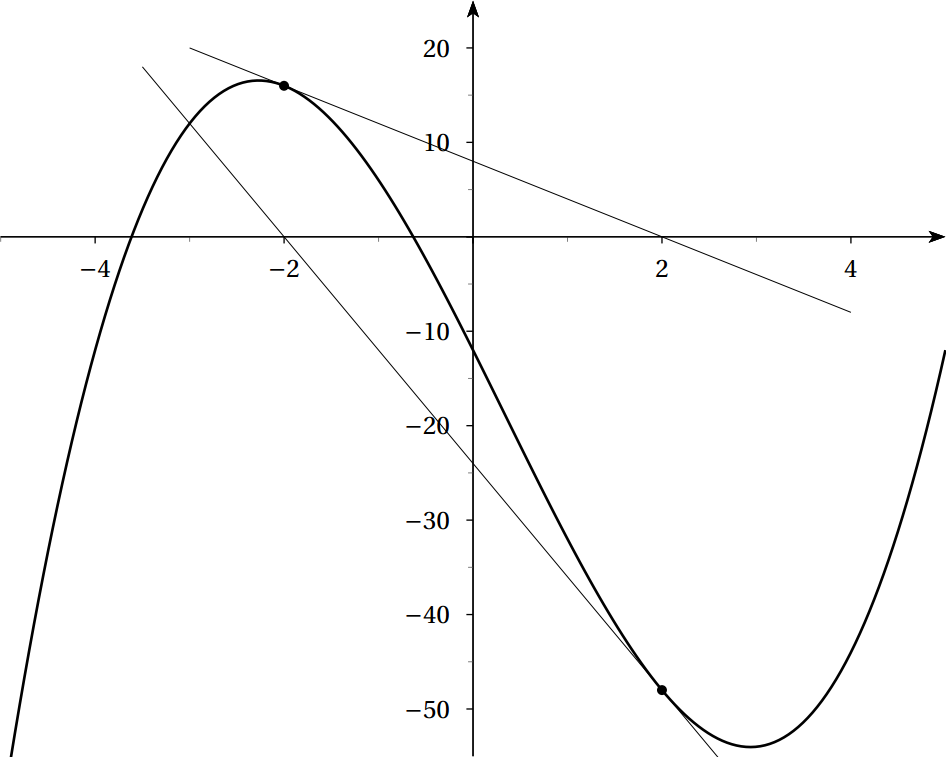
\includegraphics[width=.48\textwidth]{images/fig2}
\end{center}
%\begin{center}
%\psset{xunit=1.0cm,yunit=.1cm,
%algebraic=true,dimen=middle,dotstyle=*,dotsize=3pt 0,linewidth=0.3pt,arrowsize=3pt 2,arrowinset=0.25}
%\begin{pspicture*}(-5.,-55.)(5.,25.)
%%\multips(0,-50)(0,10.0){9}{\psline[linestyle=dashed,linecap=1,dash=1.5pt 1.5pt,linewidth=0.4pt,linecolor=lightgray]{c-c}(-5.,0)(5.,0)}
%%\multips(-4,0)(2.0,0){6}{\psline[linestyle=dashed,linecap=1,dash=1.5pt 1.5pt,linewidth=0.4pt,linecolor=lightgray]{c-c}(0,-55.)(0,25.)}
%\psaxes[labelFontSize=\scriptstyle,xAxis=true,yAxis=true,Dx=2.,Dy=10.,ticksize=-2pt 0,subticks=2]{->}(0,0)(-5.,-55.)(5.,25.)
%\psplot[plotpoints=200,linewidth=.8pt]{-5.0}{5.0}{x^(3.0)-x^(2.0)-20.0*x-12.0}
%%\psset{linestyle=dotted}
%\psplot{-3.}{4.}{(8.-4.*x)/1.}
%\psplot{-3.5}{3.}{(-24.-12.*x)/1.}
%\psdots(2,-48)(-2,16)
%\end{pspicture*}
%\end{center}


\subsection*{Exercice : Avec des listes}
\setcounter{subparagraph}{0}

Lors d'une expérience on mesure un phénomène numérique au cours du temps et on dresse deux listes (de même longueur) :
\begin{itemize}
\item \texttt{V} : la liste des mesures supposées monotones, 
\item \texttt{T} : la liste des temps (en seconde, dans l'ordre croissant) correspondant à chaque mesure.
\end{itemize}
Exemple : \texttt{T=[0, 2, \ldots]} et \texttt{V=[0.5, 0.55, \ldots]} signifie que 0.5 a été mesuré à 0s, puis la valeur suivante  (0.55) a été prise à 2s etc.


\subparagraph{}\textit{Écrire une fonction \texttt{solution(valeur,V,T)}, qui renvoie un
encadrement du temps pour lequel les mesures encadrent elles-même la valeur.}

Indication :
\begin{itemize}
\item privilégiez la dichotomie,
\item déterminez les indices \texttt{i} et \texttt{j} de cet encadrement,
\item observez que le test d'arrêt de recherche de ces entiers ne dépend pas d'une précision.
\end{itemize}

\subparagraph{}\textit{Tester ce programme avec les listes : \texttt{T=[0, 2, 3, 5, 6, 8, 10]} et \texttt{V=[0.5, 0.55, 0.7, 0.9, 1, 1.5, 1.6]} avec 0.6  pour la valeur.}

\subparagraph{}\textit{Modifier votre fonction \texttt{solution} afin de gérer (par un message d'erreur) le cas où il n'y a pas d'encadrement possible car \texttt{valeur} serait incompatible.}

\end{multicols}




